% Options for packages loaded elsewhere
\PassOptionsToPackage{unicode}{hyperref}
\PassOptionsToPackage{hyphens}{url}
%
\documentclass[
]{article}
\usepackage{lmodern}
\usepackage{amssymb,amsmath}
\usepackage{ifxetex,ifluatex}
\ifnum 0\ifxetex 1\fi\ifluatex 1\fi=0 % if pdftex
  \usepackage[T1]{fontenc}
  \usepackage[utf8]{inputenc}
  \usepackage{textcomp} % provide euro and other symbols
\else % if luatex or xetex
  \usepackage{unicode-math}
  \defaultfontfeatures{Scale=MatchLowercase}
  \defaultfontfeatures[\rmfamily]{Ligatures=TeX,Scale=1}
\fi
% Use upquote if available, for straight quotes in verbatim environments
\IfFileExists{upquote.sty}{\usepackage{upquote}}{}
\IfFileExists{microtype.sty}{% use microtype if available
  \usepackage[]{microtype}
  \UseMicrotypeSet[protrusion]{basicmath} % disable protrusion for tt fonts
}{}
\makeatletter
\@ifundefined{KOMAClassName}{% if non-KOMA class
  \IfFileExists{parskip.sty}{%
    \usepackage{parskip}
  }{% else
    \setlength{\parindent}{0pt}
    \setlength{\parskip}{6pt plus 2pt minus 1pt}}
}{% if KOMA class
  \KOMAoptions{parskip=half}}
\makeatother
\usepackage{xcolor}
\IfFileExists{xurl.sty}{\usepackage{xurl}}{} % add URL line breaks if available
\IfFileExists{bookmark.sty}{\usepackage{bookmark}}{\usepackage{hyperref}}
\hypersetup{
  pdftitle={Plan de proyecto software},
  hidelinks,
  pdfcreator={LaTeX via pandoc}}
\urlstyle{same} % disable monospaced font for URLs
\usepackage{longtable,booktabs}
% Correct order of tables after \paragraph or \subparagraph
\usepackage{etoolbox}
\makeatletter
\patchcmd\longtable{\par}{\if@noskipsec\mbox{}\fi\par}{}{}
\makeatother
% Allow footnotes in longtable head/foot
\IfFileExists{footnotehyper.sty}{\usepackage{footnotehyper}}{\usepackage{footnote}}
\makesavenoteenv{longtable}
\usepackage{graphicx}
\makeatletter
\def\maxwidth{\ifdim\Gin@nat@width>\linewidth\linewidth\else\Gin@nat@width\fi}
\def\maxheight{\ifdim\Gin@nat@height>\textheight\textheight\else\Gin@nat@height\fi}
\makeatother
% Scale images if necessary, so that they will not overflow the page
% margins by default, and it is still possible to overwrite the defaults
% using explicit options in \includegraphics[width, height, ...]{}
\setkeys{Gin}{width=\maxwidth,height=\maxheight,keepaspectratio}
% Set default figure placement to htbp
\makeatletter
\def\fps@figure{htbp}
\makeatother
\setlength{\emergencystretch}{3em} % prevent overfull lines
\providecommand{\tightlist}{%
  \setlength{\itemsep}{0pt}\setlength{\parskip}{0pt}}
\setcounter{secnumdepth}{-\maxdimen} % remove section numbering

\title{Plan de proyecto software}
\author{}
\date{}

\begin{document}
\maketitle

\hypertarget{introducciuxf3n}{%
\section{Introducción}\label{introducciuxf3n}}

La finalidad de este apartado es definir el conjunto de actividades de
desarrollo que se han llevado a cabo para gestionar la construcción de
la infraestructura \emph{software} propuesta. Estas actividades se
pueden dividir en dos fases: planificación temporal y estudio de
viabilidad.

La fase de planificación temporal agrupa todas aquellas actividades que
tienen como objetivo organizar, planificar y desarrollar una serie de
tareas dentro de un marco temporal. Todas ellas definen el intervalo de
tiempo en el que se va a desarrollar el proyecto. Existen multitud de
estrategias para determinar cada una de estas actividades, en este caso,
se ha optado por emplear metodologías ágiles.

En la segunda fase, se reúnen todas y cada una de las actividades que
estudian y analizan la viabilidad económica y legal del proyecto.

\hypertarget{planificaciuxf3n-temporal}{%
\section{Planificación temporal}\label{planificaciuxf3n-temporal}}

Para llevar a cabo la planificación temporal del proyecto se ha optado
por utilizar metodologías ágiles, concretamente \emph{Scrum}.

El desarrollo se ha dividido en iteraciones (\emph{sprints}), cada una
de las cuales ha tenido una duración aproximada de 2 semanas. Cada
iteración se compone de una serie de tareas cuyo principal cometido es
incluir nuevas funcionalidades a la infraestructura.

Las tareas de cada \emph{sprint} son elaboradas en la reunión que se
establece al terminar la iteración anterior. Además de planificar las
tareas de la siguiente iteración, se supervisan las del anterior. En
nuestro caso, las reuniones se hacían tanto con la UBU como con el
CENIEH.

Dado que el desarrollo se ha llevado a cabo en la plataforma
\emph{Github}, es importante aclarar que el término \emph{sprint}
comentado anteriormente se ve reflejado en esta plataforma como
\emph{milestone} y, cada una de sus tareas, se corresponden con las
denominadas \emph{issues}.

Además, se ha utilizado la herramienta \emph{ZenHub} para llevar a cabo
la planificación de los \emph{sprints}. Esta herramienta permite llevar
un seguimiento de cada \emph{sprint} mediante gráficos estadísticos como
\emph{burndown}. También incluye en \emph{GitHub} un nuevo atributo
denominado \emph{story points}, el cual permite asociar, a cada tarea,
una estimación del esfuerzo que se va a realizar sobre ella.

Para poder trazar un seguimiento óptimo en cada \emph{sprint}, se ha
asociado un valor temporal a cada posible valor de \emph{story points}.

\begin{longtable}[]{@{}ll@{}}
\caption{Relación entre esfuerzo (\emph{story point}) y
tiempo.}\tabularnewline
\toprule
Story points & Estimación temporal\tabularnewline
\midrule
\endfirsthead
\toprule
Story points & Estimación temporal\tabularnewline
\midrule
\endhead
1 & \textless{} 1h\tabularnewline
2 & 1h - 2h\tabularnewline
3 & 2h - 4h\tabularnewline
5 & 4h - 8h\tabularnewline
8 & 8h - 16h\tabularnewline
13 & 16h - 24h\tabularnewline
21 & 1d - 3d\tabularnewline
40 & 3d - 7d\tabularnewline
\bottomrule
\end{longtable}

A continuación, se describen brevemente cada uno de los \emph{sprints}
ejecutados durante el desarrollo del proyecto.

\hypertarget{sprint-0-28022020---13032020}{%
\subsection{\texorpdfstring{\emph{Sprint} 0 (28/02/2020 -
13/03/2020)}{Sprint 0 (28/02/2020 - 13/03/2020)}}\label{sprint-0-28022020---13032020}}

Cuando se llevó a cabo la reunión de planificación de este primer
\emph{sprint}, llevaba trabajando ya con el CENIEH más de tres semanas.
Durante este periodo de tiempo, llevé a cabo multitud de tareas
relacionadas con el proyecto. Por ello, durante esta primera reunión,
mostré todos los avances que había realizado hasta la fecha para conocer
la opinión de mis dos tutores, Carlos López y Mario Juez. Tras hacer una
valoración de dichos avances, se plantearon nuevos objetivos: migrar
todo el trabajo almacenado en el repositorio local del CENIEH al
repositorio de Github, realizar un estudio detallado de las diferentes
ontologías involucradas en el proyecto (\emph{CIDOC-CRM}, \emph{ACDM} y
\emph{AO-CAT}) y mejorar mi formación en los lenguajes de programación
utilizados por la infraestructura escogida (\emph{PHP}, \emph{HTML} y
\emph{JavaScript}).

\href{https://github.com/gcm1001/TFG-CeniehAriadne/milestone/1}{Ver
listado de tareas} asociadas al \emph{Sprint} 0.

\hypertarget{sprint-1-13032020---27032020}{%
\subsection{\texorpdfstring{\emph{Sprint} 1 (13/03/2020 -
27/03/2020)}{Sprint 1 (13/03/2020 - 27/03/2020)}}\label{sprint-1-13032020---27032020}}

Los objetivos planteados para este \emph{sprint} fueron: cubrir las
nuevas necesidades del proyecto mediante el desarrollo de nuevos plugins
para \emph{Omeka}, estudiar la opción de implementar la tecnología
\emph{Docker}, avanzar con la documentación en \emph{LaTeX} y aprender a
utilizar el servicio de documentación \emph{Read the docs}.

\href{https://github.com/gcm1001/TFG-CeniehAriadne/milestone/2}{Listado
de tareas} asociadas al \emph{Sprint} 1.

\hypertarget{sprint-2-27032020---17042020}{%
\subsection{\texorpdfstring{\emph{Sprint} 2 (27/03/2020 -
17/04/2020)}{Sprint 2 (27/03/2020 - 17/04/2020)}}\label{sprint-2-27032020---17042020}}

Los objetivos planteados para este \emph{sprint} fueron: finalizar la
formación en \emph{Docker}, adaptar el diseño de la aplicación web a las
necesidades del usuario objetivo, desarrollar un nuevo plugin que
incorpore un sistema de estados para las colecciones/ítems, gestionar el
proyecto a través de ZenHub y, por último, estudiar e implementar las
prácticas software de la CI (Integración continua).

\href{https://github.com/gcm1001/TFG-CeniehAriadne/milestone/3}{Ver
listado de tareas} asociadas al \emph{Sprint} 2.

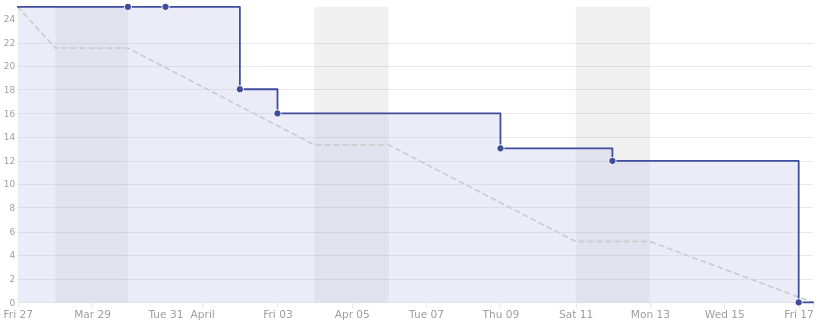
\includegraphics{../_static/images/sprint02.png}

\hypertarget{sprint-3-17042020---08052020}{%
\subsection{\texorpdfstring{\emph{Sprint} 3 (17/04/2020 -
08/05/2020)}{Sprint 3 (17/04/2020 - 08/05/2020)}}\label{sprint-3-17042020---08052020}}

Los objetivos planteados para este \emph{sprint} fueron: seguir con el
análisis e implementación de la "Integración Continua" en el proyecto,
finalizar el desarrollo del plugin "ARIADNEplus Monitor", desplegar la
infraestructura sobre el servidor del CENIEH, actualizar el fichero
README y avanzar con la documentación.

\href{https://github.com/gcm1001/TFG-CeniehAriadne/milestone/4}{Ver
listado de tareas} asociadas al \emph{Sprint} 3.

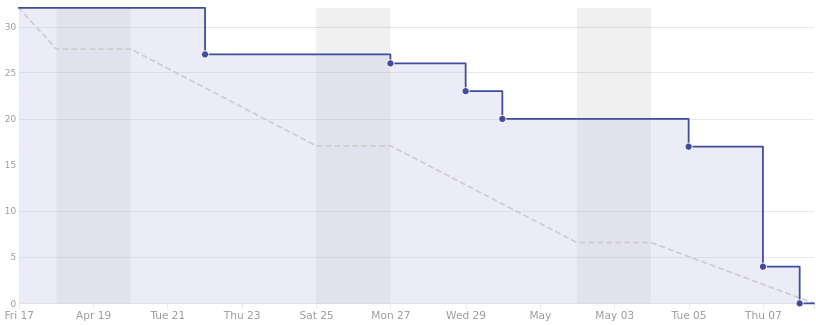
\includegraphics{../_static/images/sprint03.png}

\hypertarget{sprint-4-08052020---22052020}{%
\subsection{\texorpdfstring{\emph{Sprint} 4 (08/05/2020 -
22/05/2020)}{Sprint 4 (08/05/2020 - 22/05/2020)}}\label{sprint-4-08052020---22052020}}

Los objetivos planteados para este \emph{sprint} fueron: emplear alguna
de las herramientas propuestas para evaluar la calidad del código.
Añadir mejoras de usabilidad. Solucionar bugs de la interfaz.
Desarrollar un plugin para la gestión de tags. Mejorar el README y
seguir avanzando con la documentación.

\href{https://github.com/gcm1001/TFG-CeniehAriadne/milestone/5}{Ver
listado de tareas} asociadas al \emph{Sprint} 4.

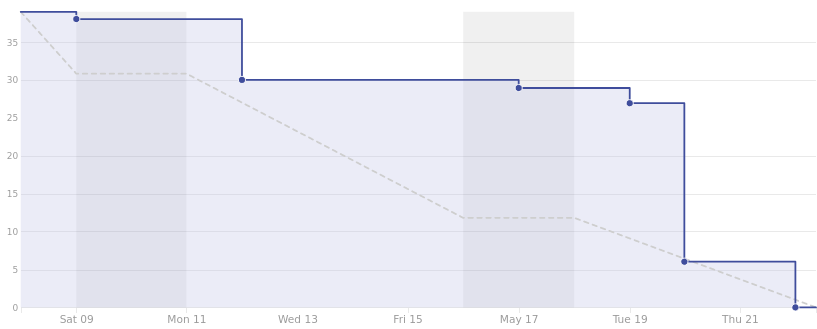
\includegraphics{../_static/images/sprint04.png}

\hypertarget{sprint-5-22052020---12062020}{%
\subsection{\texorpdfstring{\emph{Sprint} 5 (22/05/2020 -
12/06/2020)}{Sprint 5 (22/05/2020 - 12/06/2020)}}\label{sprint-5-22052020---12062020}}

Los objetivos planteados para este \emph{sprint} fueron: introducir
ciertas mejoras sobre el plugin ARIADNEplus Tracking. Crear la colección
del CENIEH en periodO. Completar la colección "CIR" con ayuda del
CENIEH. Añadir un estilo al repositorio OAI-PMH. Preparar la importación
del CIR en ARIADNEplus. Actualizar el README.md y avanzar con la
documentación.

\href{https://github.com/gcm1001/TFG-CeniehAriadne/milestone/6}{Ver
listado de tareas} asociadas al \emph{Sprint} 5.

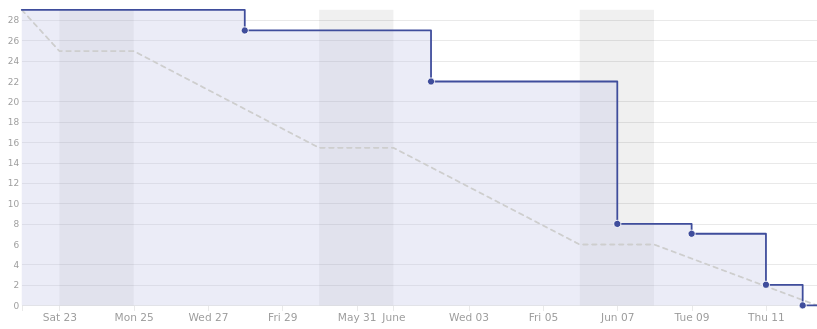
\includegraphics{../_static/images/sprint05.png}

\hypertarget{sprint-6-12062020---26062020}{%
\subsection{\texorpdfstring{\emph{Sprint} 6 (12/06/2020 -
26/06/2020)}{Sprint 6 (12/06/2020 - 26/06/2020)}}\label{sprint-6-12062020---26062020}}

Los objetivos planteados para este \emph{sprint} fueron: finalizar el
desarrollo de la aplicación, publicar la colección de periodos del
CENIEH en periodO, publicar la colección del CIR en ARIADNEplus y
continuar con la documentación (Memoria).

\href{https://github.com/gcm1001/TFG-CeniehAriadne/milestone/7}{Ver
listado de tareas} asociadas al \emph{Sprint} 6.

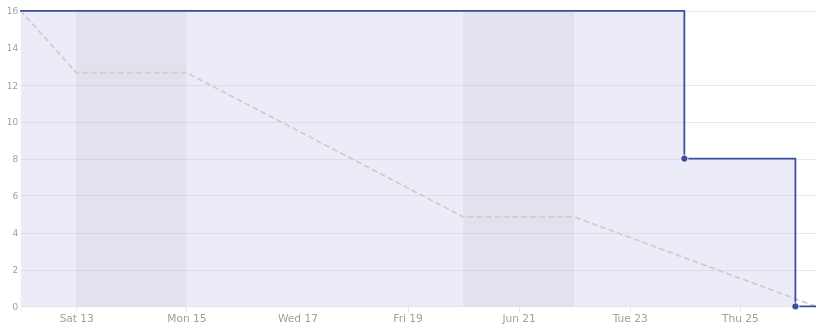
\includegraphics{../_static/images/sprint06.png}

\hypertarget{sprint-7-26062020---17072020}{%
\subsection{\texorpdfstring{\emph{Sprint} 7 (26/06/2020 -
17/07/2020)}{Sprint 7 (26/06/2020 - 17/07/2020)}}\label{sprint-7-26062020---17072020}}

Los objetivos planteados para este \emph{sprint} fueron: continuar con
el proceso de integración del CIR en ARIADNEplus. Seguir desarrollando
labores de documentación (memoria y anexos).

\hypertarget{estudio-de-viabilidad}{%
\section{Estudio de viabilidad}\label{estudio-de-viabilidad}}

\hypertarget{viabilidad-econuxf3mica}{%
\subsection{Viabilidad económica}\label{viabilidad-econuxf3mica}}

Este apartado recoge los análisis de costes y beneficios que se han
llevado a cabo para determinar la viabilidad económica del proyecto.

\hypertarget{costes}{%
\subsubsection{Costes}\label{costes}}

Los costes del proyecto se pueden clasificar en función de su
naturaleza.

\hypertarget{costes-de-personal}{%
\paragraph{Costes de personal}\label{costes-de-personal}}

El proyecto se ha llevado a cabo por un desarrollador empleado a tiempo
parcial durante 6 meses. La contratación se llevó a cabo mediante el
programa de cooperación educativa entre la Universidad de Burgos y el
consorcio CENIEH. De este acuerdo salieron dos contratos, uno de cuatro
meses de duración y otro de dos.

\begin{longtable}[]{@{}ll@{}}
\caption{Contrato prácticas curriculares}\tabularnewline
\toprule
Concepto & Coste\tabularnewline
\midrule
\endfirsthead
\toprule
Concepto & Coste\tabularnewline
\midrule
\endhead
Salario mensual neto & 400,00€\tabularnewline
Retención IRPF & 0,00€\tabularnewline
Seguridad social & 0,00€\tabularnewline
Salario mensual bruto & 400,00€\tabularnewline
Total (4 meses) & 1600,00€\tabularnewline
\bottomrule
\end{longtable}

\begin{longtable}[]{@{}ll@{}}
\caption{Contrato prácticas extracurriculares}\tabularnewline
\toprule
Concepto & Coste\tabularnewline
\midrule
\endfirsthead
\toprule
Concepto & Coste\tabularnewline
\midrule
\endhead
Salario mensual neto & 391,51€\tabularnewline
Retención IRPF & 0,00€\tabularnewline
Seguridad social & 8,49€\tabularnewline
Salario mensual bruto & 400,00€\tabularnewline
Total (2 meses) & 800,00€\tabularnewline
\bottomrule
\end{longtable}

El primer contrato, al tratarse de prácticas curriculares, queda exento
de pagar cualquier tipo de cotización. Sin embargo, en el segundo
contrato, al tratarse de prácticas extracurriculares se debe cotizar a
la seguridad social.

\hypertarget{costes-de-hardware}{%
\paragraph{\texorpdfstring{Costes de
\emph{hardware}}{Costes de hardware}}\label{costes-de-hardware}}

En este apartado se describen los costes relacionados con el
equipamiento \emph{hardware} que se ha utilizado para el desarrollo del
proyecto. Para calcular el coste amortizado, se ha tenido en cuenta que
el tiempo de uso coincide con la duración del proyecto (6 meses) y que
su vida útil gira en torno a los 5 años.

\begin{longtable}[]{@{}lll@{}}
\caption{Costes de hardware}\tabularnewline
\toprule
Concepto & Coste & Coste amortizado\tabularnewline
\midrule
\endfirsthead
\toprule
Concepto & Coste & Coste amortizado\tabularnewline
\midrule
\endhead
Ordenador portátil & 1050€ & 105,00€\tabularnewline
Monitor auxiliar & 249€ & 24.90€\tabularnewline
Servidor rack & 1400€ & 160,00€\tabularnewline
Total & 2499€ & 269,90€\tabularnewline
\bottomrule
\end{longtable}

\hypertarget{costes-de-software}{%
\paragraph{\texorpdfstring{Costes de
\emph{software}}{Costes de software}}\label{costes-de-software}}

Todo el \emph{software} utilizado para el desarrollo del proyecto era
totalmente gratuito o contaba con planes libres de pago.

\hypertarget{otros-costes}{%
\paragraph{Otros costes}\label{otros-costes}}

En la siguiente tabla se recogen los demás costes incluídos en el
proyecto.

\begin{longtable}[]{@{}ll@{}}
\caption{Otros costes}\tabularnewline
\toprule
Concepto & Coste\tabularnewline
\midrule
\endfirsthead
\toprule
Concepto & Coste\tabularnewline
\midrule
\endhead
Dominio ubucenh.es & 1,00€\tabularnewline
Internet & 136,00€\tabularnewline
Total & 137,00€\tabularnewline
\bottomrule
\end{longtable}

\hypertarget{costes-totales}{%
\paragraph{Costes totales}\label{costes-totales}}

Sumando el total de cada uno de los costes anteriores mostrados con
anterioridad, se obtiene el coste total.

\begin{longtable}[]{@{}ll@{}}
\caption{Costes totales}\tabularnewline
\toprule
Concepto & Coste\tabularnewline
\midrule
\endfirsthead
\toprule
Concepto & Coste\tabularnewline
\midrule
\endhead
Personal & 2400,00€\tabularnewline
\emph{Hardware} & 269.90€\tabularnewline
\emph{Software} & 0,00€\tabularnewline
Otros & 137,00€\tabularnewline
Total & 2806,90€\tabularnewline
\bottomrule
\end{longtable}

Se podría añadir a esta cantidad el importe de 91.935 € que la Comisión
Europea concedió al CENIEH para su integración en ARIADNEplus.

\hypertarget{beneficios}{%
\subsubsection{Beneficios}\label{beneficios}}

Con la realización de este proyecto no se pretende obtener ningún
beneficio económico o material. Cualquier persona podrá hacer uso del
material desarrollado de forma totalmente gratuita.

\hypertarget{viabilidad-legal}{%
\subsection{Viabilidad legal}\label{viabilidad-legal}}

Uno de los factores más importante a tener en cuenta en el desarrollo de
un proyecto es escoger el tipo de licencia con el que se distribuirá
cada una de sus partes. De esta forma, se define el marco legal en el
que se puede utilizar cada parte, es decir, lo que se autoriza a hacer y
lo que no.

A continuación, se asignará a cada una de las partes del proyecto,
\emph{Software} y documentación, la licencia que más se adapte a los
objetivos del proyecto.

\hypertarget{software}{%
\subsubsection{\texorpdfstring{\emph{Software}}{Software}}\label{software}}

A lo largo del proyecto se han desarrollado varios complementos
\emph{software} para una misma aplicación. En este apartado se buscará
qué licencia es la más adecuada para todos ellos.

Al hacer uso de recursos de terceros durante el desarrollo de los
complementos, la elección de la licencia se ve condicionada por las
licencias a las que estos están sometidos.

\begin{longtable}[]{@{}ll@{}}
\caption{Licencias de las dependencias utilizadas}\tabularnewline
\toprule
Dependencia & Licencia\tabularnewline
\midrule
\endfirsthead
\toprule
Dependencia & Licencia\tabularnewline
\midrule
\endhead
Zend Framework & BSD\tabularnewline
Omeka Classic & GPLv3\tabularnewline
ZipStream & MIT\tabularnewline
Leaflet Draw & MIT\tabularnewline
Sweetalert 2 & MIT\tabularnewline
Notify.js & MIT\tabularnewline
\bottomrule
\end{longtable}

Se ha considerado escoger la licencia que \emph{GNU General Public
License v3.0} (GPLv3) para cada uno de los complementos \emph{software}
desarrollados por varios motivos:

\begin{itemize}
\tightlist
\item
  Es compatible con todas las licencias mostradas en la
  \texttt{licencias}.
\item
  Al ser una licencia \emph{copyleft}, garantiza que el \emph{software}
  mantenga su carácter "libre", es decir, que pueda ser siempre
  utilizado, modificado y redistribuido por cualquier usuario.
\end{itemize}

\hypertarget{documentaciuxf3n}{%
\subsubsection{Documentación}\label{documentaciuxf3n}}

En el caso de la documentación (memoria y anexos), se ha optado por
utilizar la versión más sencilla de las licencias \emph{Creative
Commons}\footnote{"Creative Commons." \url{https://creativecommons.org/}},
que es conocida como ́*Creative Commons Attribution 4.0 International*
(CC BY 4.0).

Esta licencia es bastante permisiva ya que autoriza a realizar cualquier
tipo de operación sobre el documento involucrado, esté o no modificado,
sea o no comercial, siempre y cuando se cite al autor.

Existen otras versiones más restrictivas, sin embargo, nuestra intención
es dar la mayor libertad posible sobre el material ofrecido en este
proyecto.

\end{document}
